\documentclass{article}
\usepackage[spanish]{babel}
\usepackage{graphicx}
\usepackage{listings}
\setlength{\parindent}{0pt}
\setlength{\parskip}{3mm}
\usepackage[numbers]{natbib}
\usepackage{color}
\definecolor{dkgreen}{rgb}{0,0.6,0}
\definecolor{gray}{rgb}{0.5,0.5,0.5}
\definecolor{mauve}{rgb}{0.58,0,0.82}

\usepackage{geometry}


\addtolength{\topmargin}{-.70in}
\addtolength{\textheight}{1in}

\lstset{ 
  backgroundcolor=\color{white},   % choose the background color; you must add \usepackage{color} or \usepackage{xcolor}; should come as last argument
  basicstyle=\footnotesize,        % the size of the fonts that are used for the code
  breakatwhitespace=false,         % sets if automatic breaks should only happen at whitespace
  breaklines=true,                 % sets automatic line breaking
  captionpos=b,                    % sets the caption-position to bottom
  commentstyle=\color{dkgreen},    % comment style
  deletekeywords={...},            % if you want to delete keywords from the given language
  escapeinside={\%}{)},          % if you want to add LaTeX within your code
  extendedchars=true,              % lets you use non-ASCII characters; for 8-bits encodings only, does not work with UTF-8
  firstnumber=1,                % start line enumeration with line 1000
  frame=single,	                   % adds a frame around the code
  keepspaces=true,                 % keeps spaces in text, useful for keeping indentation of code (possibly needs columns=flexible)
  keywordstyle=\color{blue},       % keyword style
  language=Octave,                 % the language of the code
  morekeywords={*,...},            % if you want to add more keywords to the set
  numbers=left,                    % where to put the line-numbers; possible values are (none, left, right)
  numbersep=5pt,                   % how far the line-numbers are from the code
  numberstyle=\tiny\color{gray}, % the style that is used for the line-numbers
  rulecolor=\color{black},         % if not set, the frame-color may be changed on line-breaks within not-black text (e.g. comments (green here))
  showspaces=false,                % show spaces everywhere adding particular underscores; it overrides 'showstringspaces'
  showstringspaces=false,          % underline spaces within strings only
  showtabs=false,                  % show tabs within strings adding particular underscores
  stepnumber=1,                    % the step between two line-numbers. If it's 1, each line will be numbered
  stringstyle=\color{mauve},     % string literal style
  tabsize=2,	                   % sets default tabsize to 2 spaces
  title=\lstname                  % show the filename of files included with \lstinputlisting; also try caption instead of title
}
\title{
Tarea 2
}
\author{5280}
\date{\today}

\begin{document}

\maketitle


\section*{Introducción}

En este trabajo se realizan mediciones sobre los algoritmos para grafos de NetworkX \citep{networkx}:

\begin{itemize}
\item \textit{betweenness\_centrality}: Ofrece una medida de centralidad de un grafo, la cual devuelve como un diccionario de nodos, con la medidad de centralidad. Puede usarse en grafos dirigidos y no dirigidos.

\item \textit{maximal\_matching}: Devuelve un conjunto de nodos máximo conjunto posible de aristas independientes, que no tienen nodos en común. 

\item \textit{greedy\_color}: Colorea los nodo usando diferentes estrategias. Devuelve un diccionario con claves que representan nodos y valores que representan la coloración. Puede emplearse en grafos dirigidos y no dirigidos.

\item \textit{make\_max\_clique\_graph}: Devuelve el subgrafo más grande que encuentra. Debe usarse en grafos no dirigidos.
\item \textit{strongly\_connected\_components}: Se utiliza para grafos dirigidos. Devuelve un generador de conjunto de nodos, uno por cada componente fuertemente conectado. 
\end{itemize}

A los cuatro primeros algoritmos se les puede pasar como parámetro grafos no dirigidos ponderados, lo que resulta conveniente pues permite emplear el mismo conjuntos de grafos para los cuatro algoritmos. El algoritmo \textit{strongly\_connected\_components} requiere grafos dirigidos, por lo que para este se emplea otro conjunto de grafos.


\section*{Generación de grafos}
Todos los grafos son generados aleatoriamente empleando las funciones \textbf{GenerateGraph} y \textbf{GenerateDiGraph}. A estas funciones se le pasan los siguientes parámetros: 

\begin{itemize}
\item \textit{nameToSave}: Prefijo de la dirección con la que se quieren guardar los grafos. El código añadirá números consecutivos a este prefijo para cada grafo, comenzando por 0.
\item \textit{Smin}: Número mínimo de nodos que tendrán los gráfos a generar.
\item \textit{Smax}: Número máximo de nodos que tendrán los gráfos a generar.
\item \textit{max\_weight}: Peso máximo que tendrán las aristas.
\item \textit{numberOfGraphs}: Cantidad de grafos a generar.
\end{itemize}

Los grafos son convertidos a \textit{DataFrame} de la librería pandas \cite{pandas} y guardados en formato \textit{.csv}.
\lstinputlisting[language=Python, firstline=12, lastline=36]{Tarea3.py} 

\section*{Medición del tiempo de ejecución}

Para cada uno de los algoritmos seleccionados se realiza una función que recibe un grafo como parámetro, ejecuta el algoritmo y devuelve el tiempo de ejecución del mismo. 

\lstinputlisting[language=Python, firstline=54, lastline=85]{Tarea3.py} 

Estas funciones son ejecutadas mediante \textbf{RunAll}, función a la que se le pasan los siguientes parámetros:
\begin{itemize}
\item \textit{runs}: Número de veces que se quieren ejecutar los algoritmos.
\item \textit{numAlgorithms}: Cantidad de algoritmos a emplear.
\item \textit{numGraphs}: Cantidad de grafos que se va a correr para cada algoritmo.
\item \textit{name}: Formato del nombre con el que fueron guardados los grafos no dirigidos.
\item \textit{nameDi}: Formato de nombre con el que fueron guardados los grafos dirigidos.
\item \textit{matrix}: Este parámetro es un diccionario vacío cuyos índices son los números del 0 al 24.
\end{itemize}

\lstinputlisting[language=Python, firstline=115, lastline=146]{Tarea3.py} 

Este código crea una lista con las 25 combinaciones de algoritmo-grafo y para cada repetición cambia la ubicación de los elementos de la lista para garantizar la aleatoricidad del proceso. Una vez terminadas todas las mediciones, son guardadas en el archivo \textit{Matrix.csv}

\section*{Cálculo de parámetros}

Con la función \textbf{MediaDesv} se calcula la media y la desviación estándar para cada algoritmo. Esta función extrae además el número de nodos y aristas de los grafos creados, información necesaria para la creación de las gráficas de dispersión.

\lstinputlisting[language=Python, firstline=148, lastline=182]{Tarea3.py} 

Estos parámetros son guardados en formato \textit{.csv} para su posterior utilización.


\section*{Histograma}

Una vez obtenidos los valores promedios de tiempo de ejecución para cada combinación algoritmo-grafo, se grafica un histograma con los resultados, empleando la librería Matplotlib\cite{matplotlib}. En la Figura 1 se observan los histogramas correspondientes a cada algoritmo.
\begin{figure}
\begin{center}
  \includegraphics[width=1\columnwidth]{histograma.eps}
\end{center}
\vspace*{-18mm}
\caption{Histograma de las medias para cada combinación algoritmo-grafo}
  \label{Figura 1} 
\end{figure}


\section*{Gráficas de dispersión}

En la Figura 2 se observa la gráfica de dispersión en la que el eje horizontal corresponde al tiempo promedio de ejecución y el eje vertical al el número de nodos del grafo. En la gráfica de dispersión de la Figura 3, el eje horizontal corresponde de igual manera al tiempo de ejecución de los algoritmos, mientras que el vertical corresponde al número de aristas de los grafos. 

Leyenda de formas:
\begin{itemize}
\item \textit{betweenness\_centrality}=rombo
\item \textit{maximal\_matching}=círculo
\item \textit{greedy\_color}=estrella
\item \textit{make\_max\_clique\_graph}=triángulo
\item \textit{strongly\_connected\_components}=cruz
\end{itemize}

Leyenda de colores:
\begin{itemize}
\item \textit{Grafo0}=amarillo
\item \textit{Grafo1}=rojo
\item \textit{Grafo2}=azul
\item \textit{Grafo3}=negro
\item \textit{Grafo4}=verde
\end{itemize}
\begin{figure}
\begin{center}
  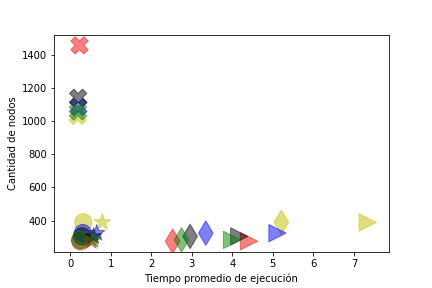
\includegraphics[width=1\columnwidth]{scatterNodes.eps}
   \end{center}
   \vspace*{-10mm}
  \caption{Gráfica de dispersión. Número de nodos respecto al tiempo de ejecución.}
  \label{Figura 2} 
\end{figure}

\begin{figure}
\begin{center}
  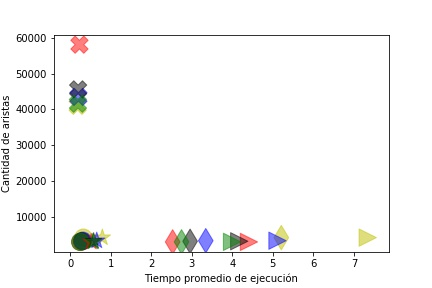
\includegraphics[width=1\columnwidth]{scatterEdges.eps}
   \end{center}
   \vspace*{-10mm}
  \caption{Gráfica de dispersión. Número de aristas respecto al tiempo de ejecución.}
  \label{Figura 3} 
\end{figure}


\section*{Conclusiones}

De manera general, pudo comprobarse que a medida que aumenta el número de nodos y/o aristas, aumenta el tiempo de ejecución de los algoritmos.





\newpage
\bibliography{Tarea3}
\bibliographystyle{plain}



\end{document}
